\documentclass[a4paper,12pt]{article}

\usepackage{natbib}
\usepackage{times}
\usepackage{graphicx,epsfig}
\usepackage[leftcaption]{sidecap}
\usepackage{subfigure} % figures can have sub chunks
\usepackage{geometry} % this maxes page usage, making the below unnecessary
% \textwidth = 6.75in
% \oddsidemargin = -0.25in
% \textheight = 10in
% \topmargin = -0.5in

\textwidth = 7.25in 
\oddsidemargin = -0.5in
\textheight = 10.25in
\topmargin = -0.75in

\usepackage{fancyhdr}
\pagestyle{fancy}
% \lhead{{\it Alan Lau}}
\chead{Demography and Culture}
\rhead{Coursework 2}
\lfoot{}
\cfoot{\thepage}
\rfoot{}
\usepackage[T1]{fontenc}
\usepackage{multirow}
\usepackage{multicol}
\usepackage{array}
\usepackage{caption}
\usepackage{hyperref}
\usepackage{graphicx}
\graphicspath{ {images/} }

\usepackage{calc}
\setlength{\parskip}{5pt}
\setlength{\parindent}{0pt}
% \addtolength{\hoffset}{0.5cm}
% \addtolength{\textwidth}{0.5cm}

% set section depth
\setcounter{tocdepth}{4}
\setcounter{secnumdepth}{5}

\newcommand{\goodgap}{%
 \hspace{\subfigtopskip}%
 \hspace{\subfigbottomskip}}

\title{Coursework 2: Demography and Culture}
% \author{Alan Lau}


\begin{document}
\maketitle

\section{Introduction}
This piece of work first attemps to replicate the effects that an increase in migratory power for individuals increases the global mean skill level shown in Powell el al (2009)'s paper, using Cace \& Bryson's (2007) evolution of communication model ("test model"). Then, we investigate the following hypothesis:

\begin{center}
    "By only allowing one subpopulation to be born with special food knowledge, it can increase the world's knowledge in the long term as the knowledge gets distributed through migration".
\end{center}

Using a more statistical-focused model, Powell et al (2009) showed that an increase in density between subpopulations, which in turns increases the probability for migration to happen and the average gloabl skill level. The experiments show that this can be replicated using a spatial model with cognititve agents. 

% - hypothesis (what you tried to do)
% - motivation (why you have done that)
% - brief background for arguments
% - cite papers for motivation (e.g. Brooks 1991)
% - present a single hypothesis you tested on your completed robot about how to improve its intelligence

\section{Approach}
Cace \& Bryson (2007) (\textit{`test model'}) provides a model that foscuses on learning through the interactions between individuals, rather than the more statistcal approach used by Powell et al (2009) (\textit{`paper model'}). In order to replicate the migration effects on the mean skill level, the \textit{test model} is modified to create four subpopulations through splitting the environment equally into four quadrants. 

Agents are assigned to their subpopulation and can only move within their subpopulation by a random distance each time. Each quadrant is separated by a space to ensure that communication cannot happen between them. A migration probability is introduced to decide whether an agent will move into another subpopulation. This is an attempt to replicate the density of subpopulation, which in essence governs how likely a gaussian random walk would land an agent in another subpopulation. Mutation is also disabled in an attempt reduce the complexity of the simulation.

% TODO: Update this about the extension
To test our hypothesis, the model is set to only allow new-borns within the top left population (\textit{q0}) to be born with special food knowledge, strictly restricting knowledge to be gained and retained through learning from migrants.

Several functions and variables are added to enable this investigation. \texttt{set-pos} and its related functions are added to establish a subpopulation setup in the form of quadrants, \texttt{migrate-or-not} and \\ \texttt{freq-of-migration} adds a migration mode.

\section{Results}
It is observed that the model reaches the optimal state faster, as the probabiliy in which an agent chooses to migrate increases, as seen in \autoref{fig:replicate}. 

\autoref{fig:test} at first demonstrates a similar peak and trough in the test on the hypothesis to the replication, but wild fluctuations are observed later in this test, resulting in a loss of talking agents, which caused the resultant skill level plummeted, rather than pleateued in \autoref{fig:replicate}.


\section{Discussion}
It is crucial to recognise that this model is inherently uncertain, due to the randomless and simulation of cognitive agents. In fact, the fluctuations seen in \autoref{fig:replicate} are most likely caused by the birth and death mechanism that simulates a real-world scenario, rather than a direct replacement for old generations in the \textit{paper model} This can also be seen sometimes when very different results are obtained under the same parameter settings.

Despite the replication was done with a more simplistic and random model, it still shows the expected trends as shown in Powell et al (2009). This demonstrates that this is a feature that works in a spatial model with uncertainties.

In the hypothesis testing, we have seen much wilder fluctuation than in the replication despite showing similar trends at first. This shows migration provide a positive effect in spreading out knowledge. However, it is speculated that withe strict limiation where only new-borns within subpopulation q0 are allowed to have prior special food knowledge, those who migrated later in life would not be able to have offsprings with such ability. This could explain the sharp drop in overall skill level as these migrated agents die, causing instability that cannot be replenished fast enough, and lowering the skill level.


\section{Conclusion}
% - on paragrape
% - restate what we tried to do and the outcome
% - results in light of the intro
We show that a replication to demonstrate that migratory power enables a higher skill level to be achieved in a shorter amount of time is possible under a spatial model is possible. However, the hypothesis where we limited new-born special food knowledge to one region strictly in the hope to show that knowledge can be spread and retained purely by migration power was unsuccessful, showing spurious fluctuations. 


\newpage
\appendix
\section{Tables and Graphs}

\begin{figure}[h]
    \centering
    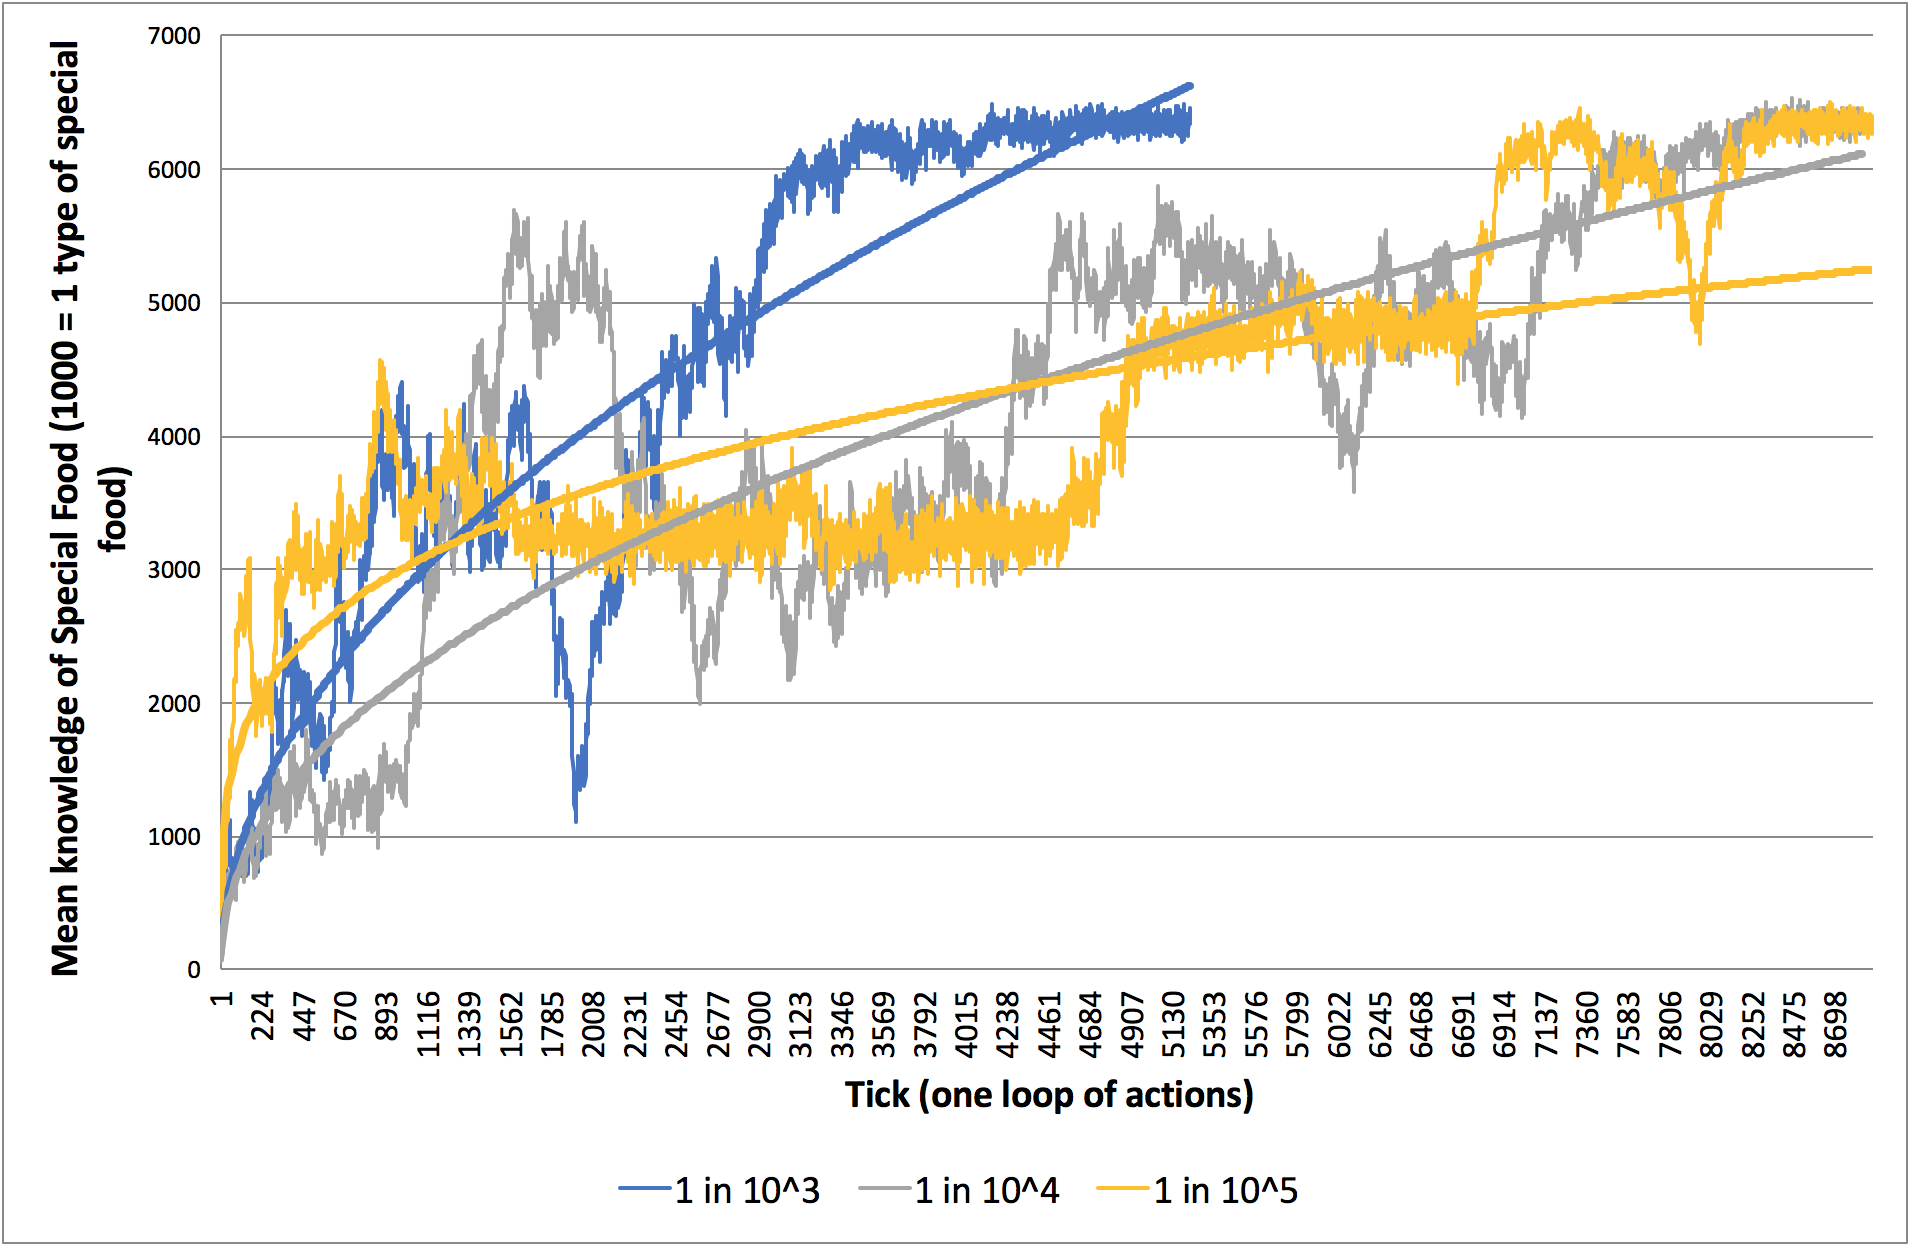
\includegraphics[width=0.8\textwidth]{replicate}
    \caption{\textit{A graph showing how three different migration probability affects global mean knowledge. It shows that the higher the probability, the faster the knowledge gap converges.}}
    \label{fig:replicate}
\end{figure}

\begin{figure}[h]
    \centering
    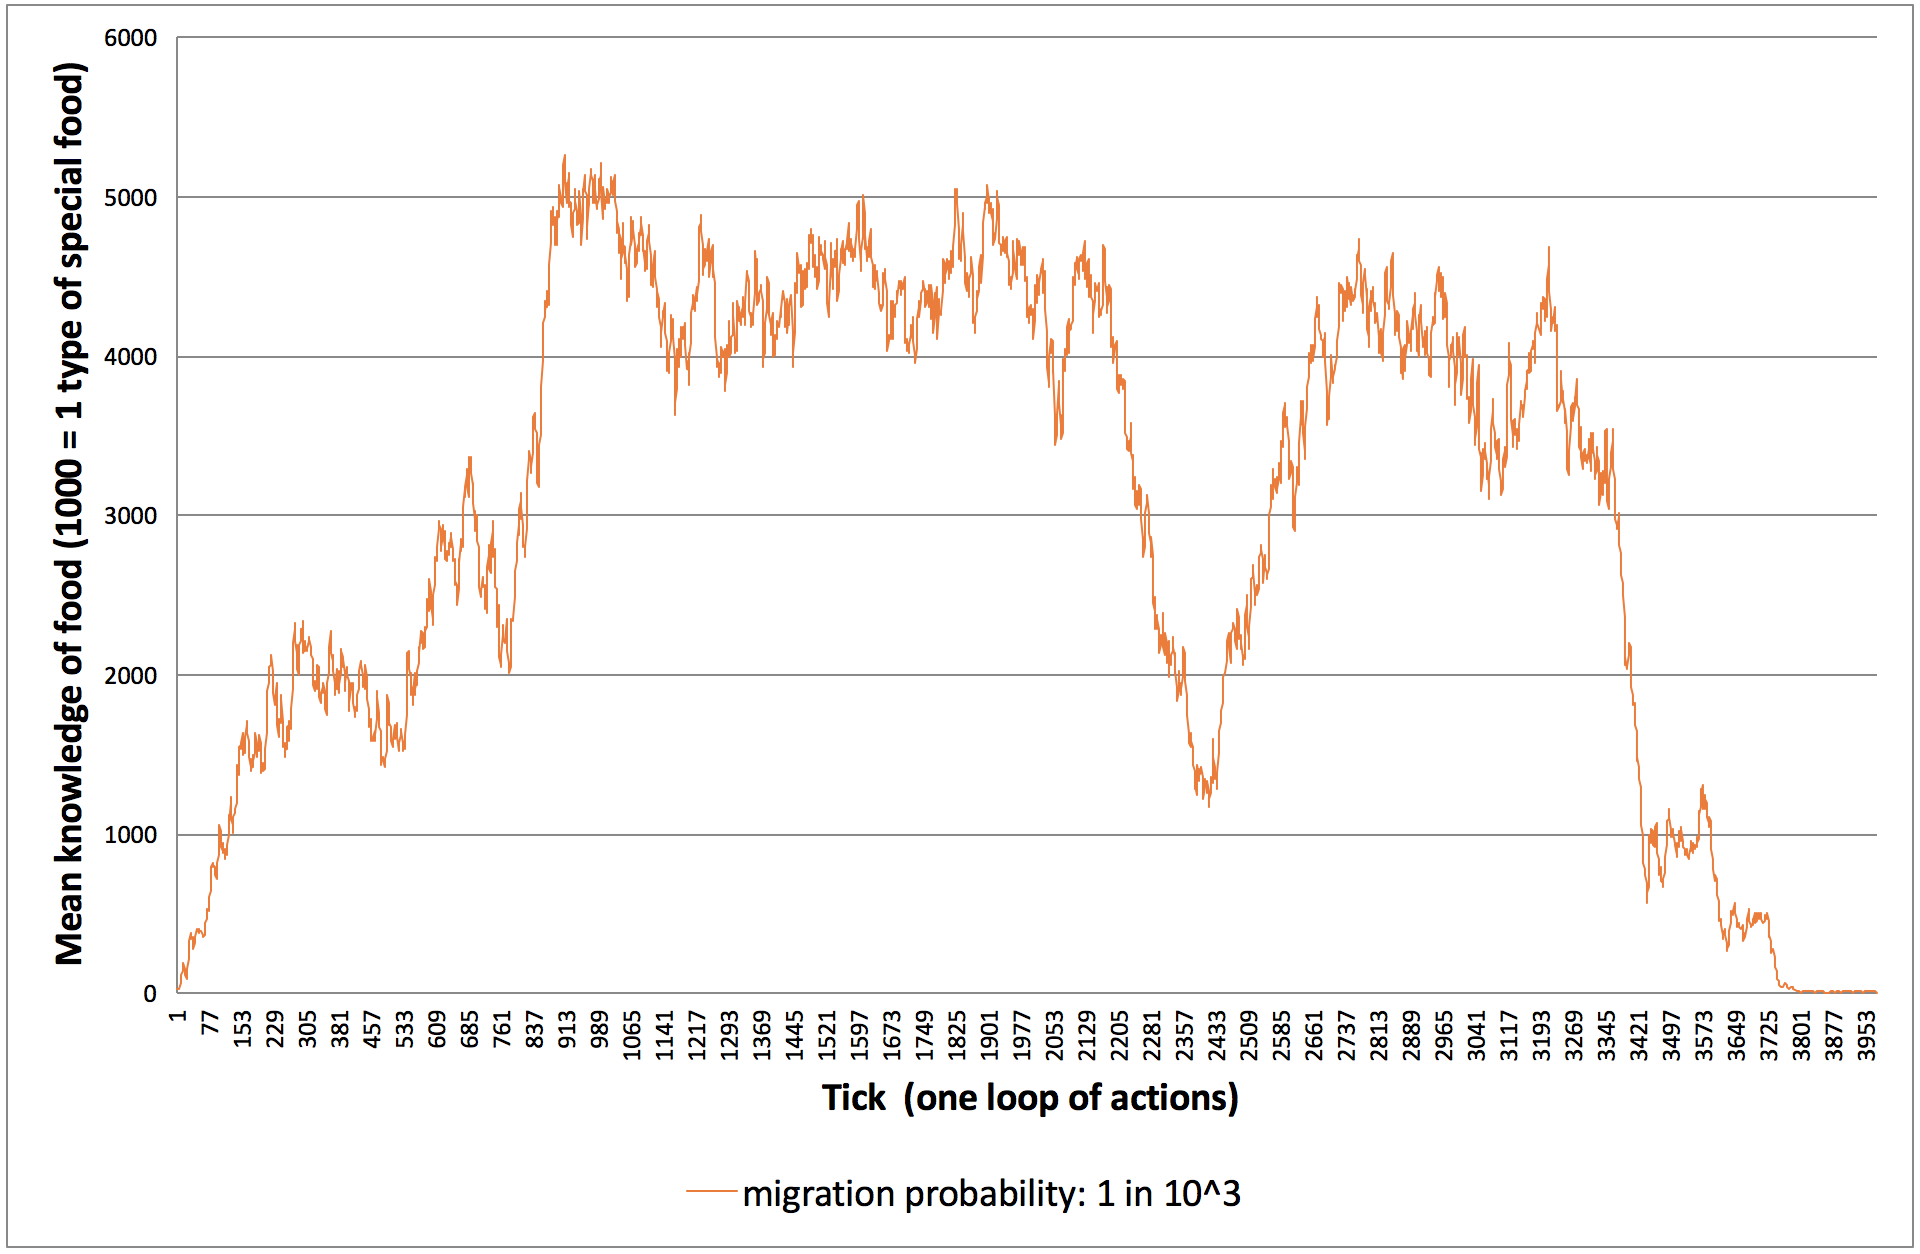
\includegraphics[width=0.8\textwidth]{test}
    \caption{\textit{A graph showing how a world with only one subpopulation who has offsprings that born with special food skills. Notice the sudden drop of knowledge caused by the lost of many skilful agents, which caused a low skill level in the end.}}
    \label{fig:test}
\end{figure}

% % TABLE - states and commands
% %%%%%%%%%%%%%%%%%%%
% {\renewcommand{\arraystretch}{1.3}%
% \parbox{\linewidth} {
    % \centering
  % \begin{tabular}{|m{0.15\textwidth}|m{0.22\textwidth}|m{0.22\textwidth}|m{0.22\textwidth}|}
        % \hline

% %%%%%%%% States
        % %\multirow{3}{*}{%}
    % \textbf{States}
      % & \texttt{FINDING\_WALL} & \texttt{FOLLOWING\_WALL} & \texttt{LOOKING\_FORWARD}
    % \\ \hline
% %%%%%%%% States 

% %%%%%%%% Commands
    % \multirow{6}{*}{\textbf{Commands}}
      % & \multicolumn{3}{c|}{\texttt{TOO\_CLOSE}} 
      % \\ %\cline{2-4}

      % & \multicolumn{3}{c|}{\texttt{TOO\_FAR}} 
      % \\ %\cline{2-4}

      % & \multicolumn{3}{c|}{\texttt{IN\_RANGE\_FAR}} 
      % \\ %\cline{2-4}

      % & \multicolumn{3}{c|}{\texttt{IN\_RANGE\_CLOSE}} 
      % \\ %\cline{2-4}

      % & \multicolumn{3}{c|}{\texttt{INTERVAL\_REACHED}} 
      % \\ %\cline{2-4}

      % & \multicolumn{3}{c|}{\texttt{TOUCH\_CONTACT}} 
      % \\ \hline
% %%%%%%%% Commands

    % \end{tabular}
% \captionof{table}{\textit{States and commands used by the robot.}}
% \label{tab:states-commands}
% }
% %%%%%%%%%%%%%%%%%%%%%%%

% \vspace{15mm}

% % TABLE - Experiment configurations
% %%%%%%%%%%%%%%%%%%%
% {\renewcommand{\arraystretch}{1.3}%
% \parbox{\linewidth} {
    % \centering
  % \begin{tabular}{|m{0.1\textwidth}|m{0.25\textwidth}|m{0.25\textwidth}|}
        % \hline

% %%%%%%%% Header
    % \textbf{Test}
      % & \textbf{Speed (degrees/sec)} & \textbf{Minimum Distance (m)} 
    % \\ \hline
% %%%%%%%% Header 

% %%%%%%%% Tests 
    % Test 1-1 & 200 & 0.2
    % \\ \hline

    % Test 1-2 & 200 & 0.3
    % \\ \hline

    % Test 1-3 & 200 & 0.4
    % \\ \hline

    % Test 2-1 & 400 & 0.2
    % \\ \hline

    % Test 2-2 & 400 & 0.3
    % \\ \hline
      
    % Test 2-3 & 400 & 0.4
    % \\ \hline

    % Test 3-1 & 600 & 0.2
    % \\ \hline

    % Test 3-2 & 600 & 0.3
    % \\ \hline
      
    % Test 3-3 & 600 & 0.4
    % \\ \hline
% %%%%%%%% Commands

    % \end{tabular}
% \captionof{table}{\textit{The different test parameter combinations. Note that variables depending on the minimum distance, i.e.} \texttt{CONCAVE\_WALL\_THRESHOLD} \textit{and} \texttt{CONVEX\_WALL\_THRESHOLD}.}
% \label{tab:exp-config}
% }
% %%%%%%%%%%%%%%%%%%%%%%%



% % TABLE - Experiment info
% %%%%%%%%%%%%%%%%%%%
% {\renewcommand{\arraystretch}{1.3}%
% \parbox{\linewidth} {
    % \centering
    % \begin{tabular}{|m{0.1\textwidth}|m{0.2\textwidth}|m{0.2\textwidth}|m{0.25\textwidth}|m{0.1\textwidth}|}
        % \hline

% %%%%%%%% Header
        % \textbf{Test} & \textbf{Mean time (sec)} & \textbf{Mean collisions / run} & \textbf{Mean missed corners / run} & \textbf{Success rate (\%)}
        % \\ \hline
% %%%%%%%% Header 

% %%%%%%%% Averages 
        % Test 1-1 & 139.86 & 1.67 & 0.33 & 100\%
        % \\ \hline

        % Test 1-2 & 129.63 & 1 & 0.67 & 100\%
        % \\ \hline

        % Test 1-3 & 125.5 & 0.33 & 1.4 & 100\%
        % \\ \hline

        % Test 2-1 & 88.83 & 6.67 & 0.67 & 100\%
        % \\ \hline

        % Test 2-2 & 70.18 & 2 & 0.67 & 100\%
        % \\ \hline
          
        % Test 2-3 & 69.63 & 0.5 & 1 & 100\%
        % \\ \hline

        % \textit{Test 3-1} & \textit{143.52} & \textit{13} & \textit{0} & \textit{33.30\%}
        % \\ \hline

        % \textit{Test 3-2} & \textit{48.57} & \textit{0} & \textit{3} & \textit{33.30\%}
        % \\ \hline
          
        % Test 3-3 & 50.35 & 1 & 2.67 & 100\%
        % \\ \hline
% %%%%%%%% Averages 

    % \end{tabular}
% \captionof{table}{\textit{Mean metrics of the experiment results. Note that Test 3-1 and Test 3-2 each only has one successful run out of three, so these are the values obtained for the successful run, rather than an average.}}
% \label{tab:exp-info}
% }
% %%%%%%%%%%%%%%%%%%%%%%%

% \vspace{10mm}

% FIG - navigation course 
% \begin{figure}[h]
    % \centering
    % 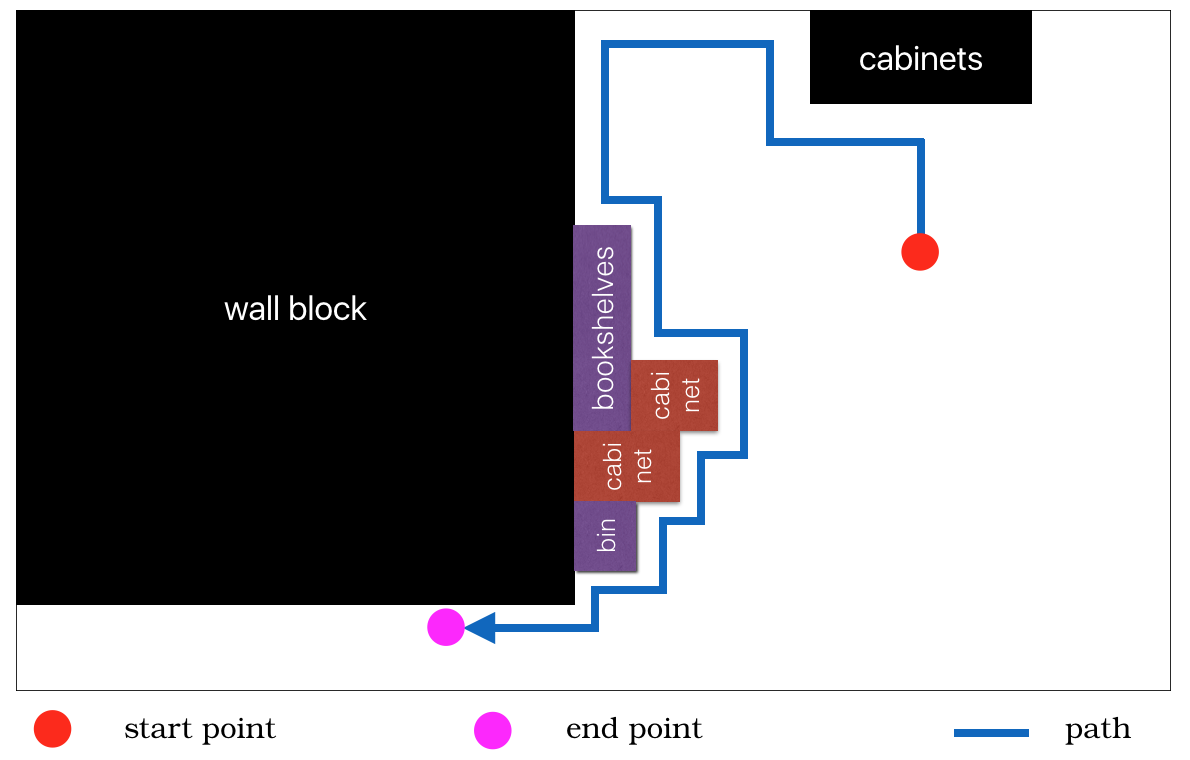
\includegraphics[width=0.8\textwidth]{path}
    % \caption{\textit{A bird's-eye view of the course setup used to develop and test the robot against our hypothesis.}}
    % \label{fig:course}
% \end{figure}

% FIG - test average time 
% \begin{figure}[h]
    % \centering
    % 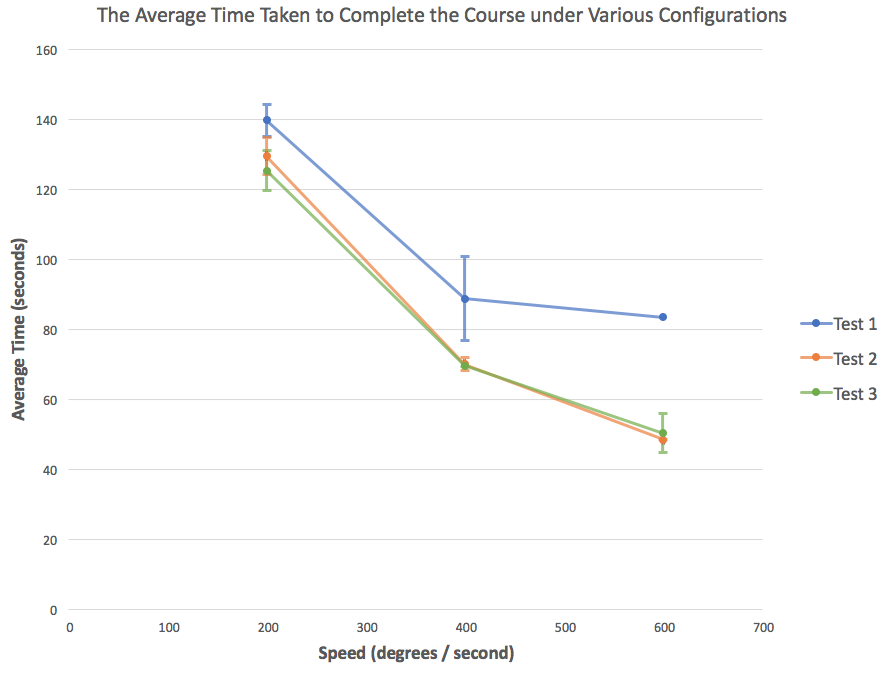
\includegraphics[width=0.8\textwidth]{time-avg}
    % \caption{\textit{We plot the average value out of the three runs, and the standard deviation bar using the sample for each configuration. Some configurations, namely, Test 1-3 and Test 3-2, failed on one or more test runs, hence a standard deviation bar is not available.}}
    % \label{fig:time-avg}
% \end{figure}

% FIG - robot
% \begin{figure}[h]
    % \centering
    % \includegraphics[width=0.8\textwidth]{robot}
    % \caption{\textit{Our robot design - a sonar sensor (`head') is attached to a motor which enables a 180-degree view (looking forward, right and left), and is mounted at a high position to capture big obstacles. Two touch sensors (`bumper') are attached in a lower position to detect low-lying obstacles and collisions. The intelligence relies heavily on the readings from the head, as we view collision as unintelligent and should be avoided. Our robot can be more intelligent by alter the motor speed if we detect that there is a wall ahead and closely monitor the wall in front and turn in time. Also, more sensors, such as a gyroscope can be used to detect the rotation angle so that a hard-coded rotation factor will not be required. }}
    % \label{fig:robot}
% \end{figure}

\end{document}
